\documentclass{article}
\usepackage[letterpaper,top=2.5cm,bottom=2.5cm,left=2.5cm,right=2.5cm,marginparwidth=1.75cm]{geometry}

\usepackage{amsmath}
\usepackage{graphicx}
\usepackage{listings}
\usepackage{xcolor}
\usepackage{alltt}
\usepackage{bm}

\title{ECE-365 Final Review}
\author{Jake Sigman}
\date{}

\definecolor{codegreen}{rgb}{0,0.6,0}
\definecolor{codegray}{rgb}{0.5,0.5,0.5}
\definecolor{codepurple}{rgb}{0.58,0,0.82}
\definecolor{backcolour}{rgb}{0.95,0.95,0.92}

\lstdefinestyle{mystyle}{
    backgroundcolor=\color{backcolour},
    commentstyle=\color{codegreen},
    keywordstyle=\color{magenta},
    numberstyle=\tiny\color{codegray},
    stringstyle=\color{codepurple},
    basicstyle=\ttfamily\footnotesize,
    breakatwhitespace=false,
    breaklines=true,
    captionpos=b,
    keepspaces=true,
    numbers=left,
    numbersep=5pt,
    showspaces=false,
    showstringspaces=false,
    showtabs=false,
    tabsize=2
}

\lstset{style=mystyle}

\begin{document}

\maketitle

\section*{Algorithm Strategies}
\subsection*{Greedy Algorithms}
\begin{itemize}
    \item Make a sequence of choices such that each choice seems to be the best choice possible at the time that you make it.
    \item \textbf{Locally optimal} choices are being made, with the hope of finding a \textbf{globally optimal} choice.
    \item If you need an algorithm guaranteed to find an optimal solution, then you need to prove that the algorithm is optimal.
    \item \textbf{The Coin-Changing Problem}
    \begin{itemize}
        \item Make change for a specified amount of money using the smallest number of coins possible.
        \item This example of a greedy algorithm will lead to the best possible solution. This wouldn't work for currencies with non-standard values.
    \end{itemize}
    \item \textbf{The Simple Scheduling Problem}
    \begin{itemize}
        \item Involves a set of jobs with a set of running times. Assume that a single processor is available.
        \item Once a job runs, it must run until completion, the goal is to schedule jobs in order to achieve the minimum average completion time.
        \item An optimal solution is to sort the jobs in terms of their running time, and schedule them in that order. This is guaranteed to be optimal, however it is not the only optimal solution.
    \end{itemize}
    \item \textbf{Huffman Code}
    \begin{itemize}
        \item Huffman code is a very popular compression algorithm.
        \item Consider a file that contains \(C\) distinct types of characters. A system that uses the same number of bits per character requires at least \(\log C\) bits per character.
        \item ASCII uses 8 bits per character, although really only 7 would be necessary for standard ASCII. Standard ASCII encodes 128 distinct characters, of which about 100 are printable.
        \item Huffman codes save about 25\% of space for large files, and can save up to 50\% and 60\% on many large data files.
        \item Let's say we take seven distinct characters: ``a'', ``e'', ``i'', ``s'', ``t'', space, and newline. If the same number of bits were used for each character, 3 bits per character would be required.
    \end{itemize}
    \begin{center}
    \begin{tabular}{|c c c c|}
    \hline
    Character & Code & Frequency & Total Bits \\ [0.5ex]
    \hline\hline
    a & 000 & 10 & 30 \\
    e & 001 & 15 & 45 \\
    i & 010 & 12 & 36 \\
    s & 011 & 3 & 9 \\
    t & 100 & 4 & 12 \\
    space & 101 & 13 & 39 \\
    newline & 110 & 1 & 3 \\
    Total & & & \textbf{174} \\
    \hline
    \end{tabular}
    \end{center}
    \begin{itemize}
        \item These encodings can be represented with a type of binary tree known as a \textbf{trie}. In a trie, left branches represent the bit 0, right branches represent the bit 1, and characters are indicated by the leaves.
        \item Some sources allow the branches of a trie to represent more general characters, or allow internal nodes to represent characters, but this is not necessary. Below is the trie with standard encoding.
        \begin{center}
        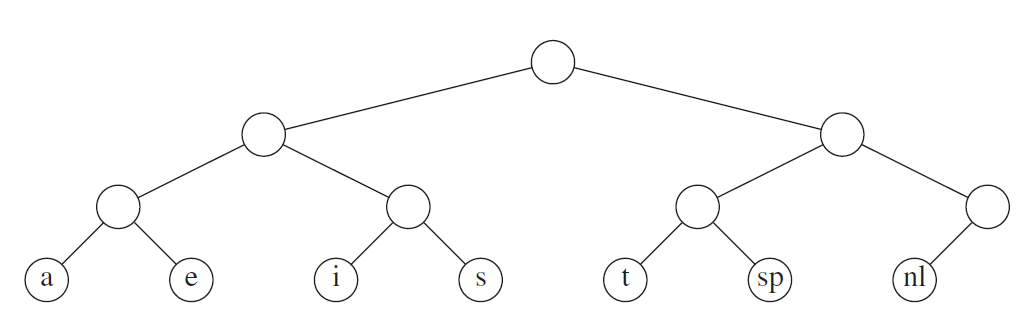
\includegraphics[scale=0.5]{trie1}
        \end{center}
        \item This is clearly not the most efficient encoding. Note that the only character with a code that starts with 11 is the newline, so the following zero does not provide useful information. An optimal trie will always be a full binary tree. Below is an image of a slightly better trie.
        \begin{center}
        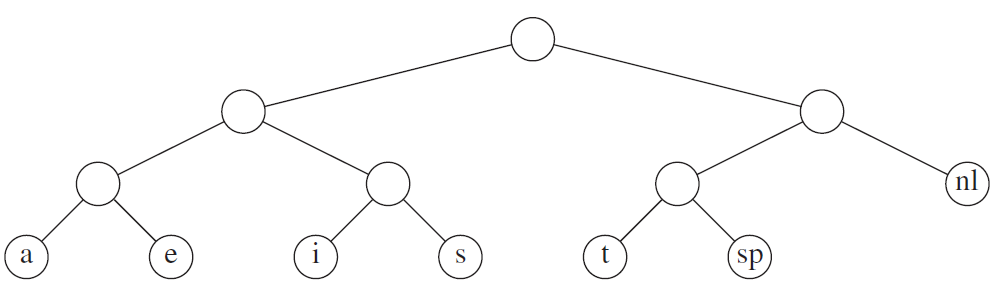
\includegraphics[scale=0.5]{trie2}
        \end{center}
        \item Any encoding in which no character code is a prefix of another character code is known as a \textbf{prefix code}. Forcing a trie to indicate each distinct character as a leaf ensures that the trie represents a prefix code. The goal of Huffman coding is to find the \textbf{optimal trie}. The trie below requires only 146 bits to encode the file.
        \begin{center}
        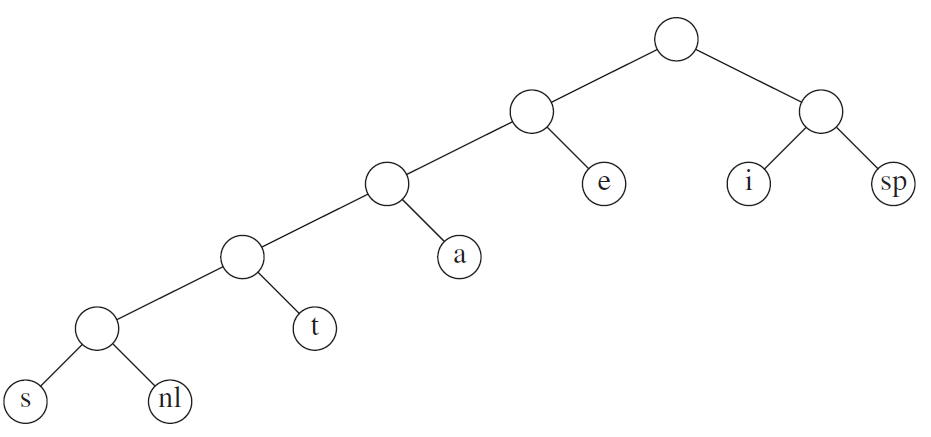
\includegraphics[scale=0.5]{trie3}
        \end{center}
    \end{itemize}
    \begin{center}
    \begin{tabular}{|c c c c|}
    \hline
    Character & Code & Frequency & Total Bits \\ [0.5ex]
    \hline\hline
    a & 001 & 10 & 30 \\
    e & 01 & 15 & 30 \\
    i & 10 & 12 & 24 \\
    s & 00000 & 3 & 15 \\
    t & 0001 & 4 & 16 \\
    space & 11 & 13 & 26 \\
    newline & 00001 & 1 & 5 \\
    Total & & & \textbf{146} \\
    \hline
    \end{tabular}
    \end{center}
    \begin{itemize}
        \item There can be many possible prefix codes that tie for optimal. In general, if each character \(c_i\) occurs \(f_i\) times, and is at depth \(d_i\) in the trie, then the cost of using the code to encode the file is equal to \(\sum_i d_i*f_i\)
    \end{itemize}
    \item \textbf{Huffman's Algorithm}
    \begin{itemize}
        \item A greedy algorithm for finding the optimal trie.
        \item Let's say that the number of distinct characters in a text file to be compressed is \(C\), Huffman's Algorithm maintains a forest of tries, the weight of each trie is equal to the sum of the frequencies of its leaves.
        \item You start with \(C\) single-node tries representing each of the characters, then through each of \(C-1\) iterations, we pick the two tries \(T_1\) and \(T_2\) with the smallest weights and form another trie with a new root and \(T_1\) and \(T_2\) as subtrees.
        \item There can only be one trie remaining, and that trie is the trie containing the optimal prefix encoding. Below is the pseudocode.
\begin{verbatim}
Huffman ( Set-of-characters C )
  initialize Q as empty priority queue
  for each character c in C
    create a single-node trie T
    T.data ← c
    T.frequency ← c.frequency
    Insert(Q, T)
  loop |C| - 1 times
    T1 ← DeleteMin(Q)
    T2 ← DeleteMin(Q)
    create a new trie T
    T.left ← T1
    T.right ← T2
    T.frequency ← T1.frequency + T2.frequency
    Insert(Q, T)
  return DeleteMin(Q)
\end{verbatim}
    \end{itemize}
\end{itemize}
\subsection*{Divide-And-Conquer Algorithms}
\begin{itemize}
    \item Applicable when a program can be broken down into parts that can be solved with a similar algorithm to the original problem. Solutions can be combined to form a final solution.
    \item The smaller parts are typically solved with \textbf{recursion}, and there must be a base case for which the recursive call does not apply.
    \item \textbf{Tower of Hanoi}
    \begin{itemize}
        \item This puzzle consists of three sticks and disks that can be placed on these sticks. At the beginning all the disks are on one stick, arranged from largest to smallest. The goal is to move the disks from the starting stick to a designated destination stick with the following rules.
        \begin{enumerate}
            \item Only one disk can be moved at a time.
            \item You can only lift the top disk off a stick.
            \item You can never place a larger disk on top of a smaller disk.
        \end{enumerate}
        \item We can move \(N\) disks from the source stick to the destination stick with the following steps.
        \begin{enumerate}
            \item Move \(N-1\) disks from the source stick to the auxillary stick (recursive).
            \item Move the largest disk from the source stick to the destination stick.
            \item Move \(N-1\) disks from the auxillary stick to the destination stick (recursive).
        \end{enumerate}
        \item The pseudocode for solving the Tower of Hanoi is below.
\begin{verbatim}
void Tower(int n, string src, string dst, string aux) {
  if (n == 1)
    cout << "Move from " << src << " to " << dst << "\n";
  else {
    Tower(n-1, src, aux, dst);
    cout << "Move from " << src << " to " << dst << "\n";
    Tower(n-1, aux, dst, src);
  }
  return;
}
\end{verbatim}
    \end{itemize}
\end{itemize}
\subsection*{Dynamic Programming Algorithms}
\begin{itemize}
    \item Sometimes the recursive approach can be slower, this is where dynamic programming comes in use. While it may use more memory, it takes less time.
    \item Dynamic programming has a lot of practicality in computing a Fibonacci sequence which has exponential time complexity.
    \item \textbf{Bottom-Up Dynamic Programming}
    \begin{itemize}
        \item This version of implementing the Fibonacci sequence uses linear memory, but this version is more readable, and is easily expandable to functions that rely on previous values.
        \item Computed values are being stored in an array, and each newly computed value depends on other values that have already been computed.
\begin{verbatim}
Fibonacci( integer N )
  if N ≤ 2
    return 1
 
  Fib[1] ← 1
  Fib[2] ← 1
  Loop i from 3 to N
    Fib[i] ← Fib[i-1] + Fib[i-2]
 
  return Fib[n]
\end{verbatim}
    \end{itemize}
    \item \textbf{Top-Down Dynamic Programming}
    \begin{itemize}
        \item This version of implementing the Fibonacci sequence is recursive, but this version executes in linear time. The array ``known'' could be a global array, and the array must be large enough to hold \(N\) values, all initialized to ``unknown''.
        \item Computed values are being stored in an array after they are computed via recursive calls. The start of each recursive routine checks to see if the desired value has already been computed. This use of an array or matrix is called \textbf{memoization}.
\begin{verbatim}
Fibonacci( integer N )
  if known[N] != unknown
    return known[N]
 
  if N ≤ 2
    v ← 1
  else
    v ← Fibonacci(N-1)+Fibonacci(N-2)
 
  known[N] ← v
  return v
\end{verbatim}
    \end{itemize}
    \item \textbf{Longest Common Subsequence Problem}
    \begin{itemize}
        \item Another use of dynamic programming is in solving the longest common subsequence problem. Consider a string \(X=x_1x_2x_3\,\hdots\,x_n\). A subsequence of \(X\) is any string \(Z=z_1z_2z_3\,\hdots\,z_k\) for which there exists a strictly increasing sequence \(i_1, i_2\,\hdots\,i_k\) such that for all \(j=1,2\,\hdots\,k\) it is true that \(z_j=x_{i_j}\).
        \item Now consider two strings, \(X\) as defined above and \(Y=y_1y_2y_3\,\hdots\,y_m\). The longest common subsequence problem asks us to determine the longest string, \(Z\) that is a subsequence of both \(X\) and \(Y\).
        \item To solve this problem, a matrix \(M\) with \(n+1\) rows and \(m+1\) columns will be used.
        \begin{itemize}
            \item \(M[i,j]\) represents the length of the longest common subsequence of the strings \(x_1x_2x_3\,\hdots\,x_i\) and \(y_1y_2y_3\,\hdots\,y_j\).
            \item If we want to fill in a particular slot \(M[i,j]\) and we have already filled in all the slots above this slot and all the slots to the left of this slot in the current row, we can say that if \(x_i==y_j\), then \(M[i,j]\) must equal \(M[i-1,j-1]+1\).
            \item Otherwise, \(M[i,j]\) will be the maximum of \(M[i-1,j]\) and \(M[i,j-1]\).
        \end{itemize}
        \item At the end of the algorithm, the length of the longest common subsequence is stored at the bottom right of the matrix in \(M[n,m]\). This is a Bottom-Up approach. The pseudocode is below.
\begin{verbatim}
LongestCommonSubsequence ( String X, String Y )
  n ← length(X)
  m ← length(Y)
  loop i from 0 to m
    M[0,i] ← 0
  Loop i from 0 to n
    M[i,0] ← 0
  Loop i from 1 to n
    Loop j from 1 to m
      if Xi == Yj
        M[i, j] ← M[i-1, j-1] + 1
      else if M[i-1, j] ≥ M[i, j-1]
        M[i, j] ← M[i-1, j]
      else
        M[i, j] ← M[i, j-1]
\end{verbatim}
        \item The pseudocode above fills out the matrix, but does not retrieve the maximum length or the subsequence itself. It is possible to use the matrix to do exactly this.
        \item Firstly, start at the bottom right of the matrix at position \((n,m)\).
        \item Move up, left, or both after each iteration and stop when you hit the top row or left column.
        \item If, at position \((i,j)\) it is the case that \(X_i==Y_j\), then this character is a part of the subsequence. Then append this character to the subsequence, and move up and to the left.
        \item Otherwise, decide if it required to move up one row or left one column.
        \item Below is the pseudocode for retrieving the longest common subsequence.
\begin{verbatim}
LongestCommonSubsequence ( String X, String Y, Matrix M )
  i ← length(X)
  j ← length(Y)
  subsequence ← empty string
  while i > 0 and j > 0
    if Xi == Yj
      subsequence ← Xi + subsequence
      i ← i - 1
      j ← j - 1
    else if M[i-1, j] ≥ M[i, j-1]
      i ← i - 1
    else
      j ← j - 1
\end{verbatim}
        \end{itemize}
    \end{itemize}
\subsection*{Randomized Algorithms}
\begin{itemize}
    \item These are algorithms that rely on randomness. However, modern-day computers are not capable of true randomization. There are however ways to develop pseudo-random algorithms.
    \item \textbf{Pseudo-Random Number Generators}
    \begin{itemize}
        \item All modern programming languages include routines to generate \textbf{pseudo-random} numbers. These are referred to as random number generators.
        \item In C and C++, you can use the rand() function, which returns a pseudo-random integer from 0, to RAND\_MAX.
        \item Random number generators rely on a global variable that changes each time it is used. The initial value of this global variable is called a \textbf{seed}.
        \item The entire sequence of pseudo-random numbers that are generated is determined based on this seed. It is impossible for the seed to be actually random, but all that is required is for the seed to be different every time. You can use srand("seed") to set the seed of the rand() function.
        \item Below is an example of a pseudo-random number generator.
\begin{verbatim}
unsigned long int next = 1;
 
int rand(void) {
  next = next * 1103515245 + 12345;
  return (unsigned int) (next/65536) % 32768;
}
 
void srand(unsigned int seed) {
  next = seed;
}
\end{verbatim}
        \item What makes a good random number generator? The following four characteristics. If the first three properties are not present, the result of a program relying on the generator might be too predictable.
        \begin{enumerate}
            \item The period of numbers before repitition should be long.
            \item Sequences of generated numbers should be uniformly distributed.
            \item Subsequences of generated numbers should be uncorrelated.
            \item The generator should be efficient.
        \end{enumerate}
        \item One example of a randomized algorithm is called a \textbf{skip list}.
        \begin{itemize}
            \item This involves a link list, where some nodes contain more than one link, each pointing to a different number of nodes ahead.
            \item The data structure can support insertion and search in \(O(\log N)\) time.
            \item For some algorithms, this could be more efficient than a binary search tree.
        \end{itemize}
        \item Another example of a randomized algorithm is an algorithm that checks to see if a number is prime.
        \begin{itemize}
            \item If the algorithm returns true, the number is prime with high probability. If the algorithm returns false, the number is definitely not prime.
            \item By repeating the algorithm, we can reduce the probability of error significantly.
        \end{itemize}
    \end{itemize}
\item \textbf{The 8-Queens Problem}
    \begin{itemize}
        \item Challenges us to place 8 queens on a chessboard such that no two queens are attacking eachother.
        \item Recognize that one queen has to be placed in each column, and it can backtrack as soon as two queens attack eachother. This can be scaled up to the \textbf{N-Queens Problem} using a randomized algorithm, which also happens to be a greedy algorithm.
        \item \textbf{Hill Climbing} is a search strategy that iteratively replaces the current state with its best neighboring state. When no neighbor is better than the current state, the search is finished. This can be applied to the 8-Queens Problem.
        \begin{itemize}
            \item We start by randomly placing one queen in each column.
            \item At each step, we will allow movements of any queen to any other square in the same column, therefore there will always be 56 possible moves or actions.
            \item The best neighbor is the state which has the smallest number of pairs of queens attacking eachother. If no moves improve the situation, we can allow sideways moves, which may allow us to improve the situation over time.
            \item Without sideways moves, hill climbing has a 14\% chance of success, but with 100 allowed sideways moves, hill climbing has a 94\% chance of success.
            \item If we want an algorithm to solve the 8-Queens Problem every time, we can use \textbf{Random-Restart Hill Climbing}. If the algorithm fails, simply start over until it works.
    \end{itemize}
\end{itemize}
\item \textbf{The Submarine/Number-Line Puzzle}
    \begin{itemize}
        \item Imagine a number-line, infinitely long, and somewhere on that number line, there exists a submarine which has a finite integer velocity that will never change.
        \item At every unit, you may drop one bomb at one integer location, in response you will be told that you either hit the submarine, or that you did not hit the submarine.
        \item This puzzle asks you to come up with a strategy that is guaranteed to eventually hit the submarine.
        \item The method used to solve this puzzle is an \textbf{exhaustive search}. This is a brute-force search. This search iterates through all possible pairs. It's not very efficient.
    \end{itemize}
\item \textbf{Backtracking Search}
    \begin{itemize}
        \item Backtracking search is a clever implementation of an exhaustive search, unfavorable performance.
        \item Backtracking search adds \textbf{pruning} to exhaustive search, meaning that you can sometimes skip possiblities that lead to a solution.
        \item An application of this is called a \textbf{minimax search}.
        \begin{itemize}
            \item Thie is a strategy that can be used for deterministic, turn-taking, two-player, zero-sum games of perfect information. We will label the two players playing the game as MAX and MIN, only one can win.
            \item We start by considering a hypothetical \textbf{game tree} for a simple game. Depict MAX with upward-pointing triangles, and MIN with downward-pointing triangles.
            \item A minimax search computes the minimax value of each node in a game tree as follows.
\begin{alltt}
MINIMAX (s) =
  UTILITY(s) if IS-TERMINAL(s); i.e., if s is a terminal state (leaf)
  \(\textnormal{max}\sb{a\epsilon\textnormal{ACTIONS(s)}}\) MINIMAX(RESULT(s, a)) if TO-MOVE(s) = MAX
  \(\textnormal{min}\sb{a\epsilon\textnormal{ACTIONS(s)}}\) MINIMAX(RESULT(s, a)) if TO-MOVE(s) = MIN
\end{alltt}
            \item The game tree is never stored as a data structure. The minimax decision using this function maximizes the worst-case scenario.
            \item This algorithm performs a complete depth first search of the game tree, therefore it's an example of an exhaustive search.
            \item If the maximum depth of the game tree is \(m\) and there are at most \(b\) legal moves per state, the time complexity of the search is \(O(b^m)\). The space requirement is \(O(b*m)\) if all moves are generated at once.
            \item An issue with this search is that the number of game states is exponential with respect to the number of moves. A search that adds \(\bm{\alpha}\)-\(\bm{\beta}\) \textbf{pruning} returns exactly the same move as a full minimax search. Howerver, it does not consider the majority of the nodes in the game tree in most cases.
            \item Two new search parameters need to be added.
            \begin{enumerate}
                \item \(\alpha=\) the best choice for MAX along the current path.
                \item \(\beta=\) the best choice for MIN along the current path.
            \end {enumerate}
            \item With these changes the search now becomes an \(\bm{\alpha}\)-\(\bm{\beta}\) \textbf{search}. This can allow you to search 50\% to 100\% deeper in the tree in a given amount of time.
            \item Even with \(\alpha\)-\(\beta\) pruning, it is not feasible to search entire game trees for some games. One possibility is to search a specified depth limit, at which point an \textbf{evaluation function} is applied.
            \begin{itemize}
                \item The evaluation function should order moves based on their quality, and it must be zero-sum.
                \item No non-definite win should get a score as high as a definite win, and no non-definite loss should get a score as low as a definite loss.
                \item Conventionally, evaluation functions have been manually constructed, but in recent years, they have been learned for some games using reinforcement learning.
            \end{itemize}
            \item If each move has a specified time limit, \textbf{iterative deepening} can be applied. This means that there are sequential depth-limited searches. If the time runs out in the middle of a search, it stops, and the move chosen based on the brevious depth-limited search is selected.
            \item A \textbf{transposition table} is a hash table that stores evaluations of positions that have been searched up to a particular depth. This can be used to avoid redundant searches.
        \end{itemize}
    \end{itemize}
\end{itemize}
\section*{Theoretical Computer Science}
\subsection*{Gödel's Theorem}
\begin{itemize}
    \item This is the first of two theorems, but together they are referred to as \textbf{Gödel's Incompleteness Theorems}.
    \item This was in response to David Hilbert, who was trying to prove that arithmetic was both \textbf{consistent} and \textbf{complete}.
    \begin{itemize}
        \item A complete system of arithmetic is one such that every true statement that can be expressed by the language can theoretically be proven within the language.
        \item A consistent system of arithmetic is one that does not contradict itself.
    \end{itemize}
    \item No system capable of expressing all basic facts of arithmetic can be both consistent and complete. His original proof included a very technical portion proving that symbols representing certain concepts like ``for all'' and ``there exists'' must exist.
    \item A finite number of symbols is required to represent any mathematical system, and given those symbols, it is possible to list them, first every possible one character, then two character combinations, and so on. This is called \textbf{lexographical ordering}. Some of these strings will have meaning, and some will not.
    \begin{itemize}
        \item \textbf{Propositions} are mathematical facts that can be stated using these symbols.
        \item Some will be \textbf{propositional functions} that depend on one or more variables.
    \end{itemize}
    \item \textbf{Gödel Sentences}
    \begin{itemize}
        \item \(\bm{P_n}\): The \(n^{\textnormal{th}}\) propositional function on a single variable.
        \item \(\bm{P_n(w)}\): That propositional function applied to \(w\).
        \item \(\bm{\Pi_n}\): The \(n^{\textnormal{th}}\) proof in the language according ot lexographical ordering.
        \item \(\bm{\sim\exists x\left[\Pi_x\,\textbf{proves}\,P_w(w)\right]}\): There does not exist an \(x\) such that \(\Pi_x\) proves \(P_w(w)\).
        \item When \(k\) is put into the above sentence, you get: \(\sim\exists x\left[\Pi_x\,\textnormal{proves}\,P_k(k)\right]\)
        \begin{itemize}
            \item This statement means that ``There does not exist a proof of this statement.''. If there is a proof of this statement, the statement becomes false, which is a contradiction. This means that there are certain true statements that cannot be proven.
        \end{itemize}
    \end{itemize}
\end{itemize}
\subsection*{Turing Machines}
\begin{itemize}
    \item The turing machine was invented in response to the \textbf{Entscheidungsproblem}, or decision problem. This was a challenge to mathematicians to produce a mechanical procedure that could solve all formally expressible yes/no mathematical questions. Alan Turing proved that a solution to this problem is impossible.
    \item A Turing Machine consists of a tape that is infinitely long in both directions. This tape is comprised of an infinite sequence of squares, and each square is either marked or blank. Imagine a read-write head that starts over some starting location.
    \item At most, a finite number of squares will be marked with a symbol from the alphabet, the rest will be blank.
    \item A Turing Machine consists of a finite set of possible \textbf{internal states}. One state is indicated as the \textbf{initial state} and some are final states, also known as \textbf{accepting states}.
    \item A Turing Machine consists of a \textbf{transition function} indicating a set of rules. Each rule has a very specific format: If we are in state \(x\) and read symbol \(s_1\), then write symbol \(s_2\), move one square (either left or right), and go to state \(y\). This is the only type of action a turing machine is capable of.
    \item The \textbf{power} of a Turing Machine is what is/is not possible for the Turing Machine to perform. You may not need the whole alphabet or blank cells. Limiting symbols to 0 and 1 is good enough without decreasing the power of the machine.
    \item An example of a specific rule: \(_{100}0 \rightarrow _{10101}\!\!1R\)
    \item The \textbf{Church-Turing thesis} states that any calculation that can be performed by any device is computable on a Turing Machine. This forms the formal definition of an algorithm, which is a computational process that can be reproduced by some Turing Machine. Modern computers are there for not more powerful than Turing Machines. Anything you can do in polynomial time on a modern computer, you can do in polynomial time on a Turing Machine.
    \item A \textbf{Universal Turing Machine} is a Turing Machine that can simulate all other Turing Machines. This reads from its input tape a description of a Turing Machine to emulate, the rest of the tape stores the input to this Turing Machine. Then, it simulates the specified Turing Machine and applies it to the appropriate input.
    \item Turing proposed a problem now known as the \textbf{halting problem} which is stated as follows: Devise an algorithm to decide whether the \(n^\textnormal{th}\) Turing Machine eventually halts on the \(m^\textnormal{th}\) possible output. This is known as a \textbf{decision problem}, which challenges us to find an algorithmic solution to answer a yes/no question. If such algorithm exists, the problem is said to be \textbf{decidable}, solvable, or computable. Otherwise, it is said to be \textbf{undecidable}. The halting problem is undecidable.
    \item Proving that the halting problem is undecidable can be done in two different ways.
    \begin{enumerate}
        \item Contradiction
        \begin{itemize}
            \item First, assume it is possible to solve the halting problem. You could then create a function halt(a, i) which accepts two strings representing the encoding of a Turing Machine (a) and its input (i).
            \item This function should return true if the algorithm halts on the input, and false otherwise.
            \item Consider the following function.
\begin{verbatim}
function Trouble(string s)
   if halt(s, s) == false
     return true
   else
     loop forever
\end{verbatim}
            \item If it is possible to write such function, then it must be implemented by some Turing Machine, let t be the string encoding of that Turing Machine. If you call Trouble(t), this leads to a paradox. Therefore, it is not possible to solve the halting problem.
        \end{itemize}
        \item \textbf{Diagonalization}
        \begin{itemize}
            \item Turing's proof was a bit different and used diagonalization.
            \item Consider an infinite table where the rows represent every posible valid Turing Machine, and the columns represent every possible input.
            \item If the halting problem is solvable, then we can use it to fill out a matrix M[i][j]=halt(i, j). Somewhere in this matrix there will be a Turing Machine that performs the trouble algorithm above.
            \item Turing showed that no row of this table could contain said Turing Machine, because the intersection would have a different answer.
        \end{itemize}
    \end{enumerate}
    \item Another type of Turing Machine is a \textbf{Nondeterministic Turing Machine}. For every internal state, instead of one action that is always taken, there will be a set of actions. This type of Turing Machine takes all applicable actions at once, leading to a superposition of Turing Machine configurations. As soon as any path leads to an accepting state, the entire machine stops.
\end{itemize}
\subsection*{Complexity Classes}
\begin{itemize}
    \item A complexity class defines a set of computational problems with similar Big-O time or memory bounds for deterministic or nondeterministic Turing Machines.
    \item The class \textbf{P} defines all decision problems that can be solved by a regular Turing Machine in polynomial time.
    \item The class \textbf{NP} defines all decision problems that can be solved by a nondeterministic Turing Machine in polynomial time.
    \item Anything you can do in polynomial time with a deterministic Turing Machine, you can do in polynomial time with a nondeterministic Turing Machine. This means that P is a subset of NP. However, there could be problems in NP that are not in P. This brings the \textbf{P=NP question}. The answer to this question is not known.
    \item If there is any problem that is in NP but not P, such a problem is solvable by a regular Turing Machine in theory, but only with an exponential-time algorithm. Such problems are said to be \textbf{intractable}.
    \item A \textbf{reduction} refers to the situation when an instance of one problem can be mapped to an instance of another problem. Typically, we are interested in polynomial-time reductions. If \(P_1\) can be reduced to \(P_2\) in polynomial time, you can express this as \(P_1\,\leq_p\,P_2\). You can use an algorithm that solves \(P_2\) to solve \(P_1\).
    \item The class \textbf{NP-hard} includes every decision problem for which every problem in NP can be reduced to it in polynomial time.
    \item The class \textbf{NP-complete} includes every decision problem that is in NP and for which every problem that is in NP can be reduced to it in polynomial time. Any NP-hard problem that is also NP.
    \item \textbf{Cook's Theorem}
    \begin{itemize}
        \item Stephen Cook proved that the Boolean Satisfiability Problem (SAT) is NP-complete.
        \item The problem: Given a boolean expression containing boolean variables, ands, ors, nots, and parentheses, is there any assignment of truth values that makes the expression true?
        \item To prove this, we need to prove that it is in NP, and it is in NP-hard. This can be verified by a regular Turing Machine in polynomial time. Similarly, a nondeterministic Turing Machine could try out all possible solutions simultaneously, and solve the decision problem in polynomial time, which means that SAT is in NP.
        \item To prove that it is NP-hard, there is a bit more that needs to be done. We can say that \(M\) is some nondeterministic Turing Machine consisting of a set of states (\(Q\)), an alphabet (\(\epsilon\)), an initial state (\(s\)), \(F\) accepting states, and \(\delta\) transition functions. \(M=(Q,\epsilon,s,F,\delta)\) and \(I\) is a finite string of alphabet symbols that serve as the input to the turing machine. We will being by constructing a boolean expression \(B\).
        \begin{itemize}
            \item Variables of \(B\)
            \begin{itemize}
                \item \(T_{i,j,k}\): A boolean variable set to true if an only if tape cell \(i\) contains symbol \(j\) at step \(k\) of the computation.
                \item \(n\): The size of the input, \(p(n)\) is a polynomial describing the number of computational steps. This makes \(T_{i,j,k}=O[p(n)^2]\). The problem is assumed to be NP.
                \item \(H_{i,k}\): A boolean variable that is true if and only if the read/write head at \(M\) is at tape cell \(i\) at step \(k\) of the computation.
                \item \(Q_{q,k}\): A boolean variable that is true if and only if \(M\) is in state \(q\) at step \(k\) of the computation. There are \(O[p(n)]\) such variables.
            \end{itemize}
            \item Notation
            \begin{itemize}
                \item \(\wedge\): or
                \item \(\lor\): and
                \item \(\neg\): not
            \end{itemize}
            \item Clauses of \(B\)
            \begin{itemize}
                \item \(T_{i,j,0}\) for all \(i\) and \(j\) such that the tape cell \(i\) of input \(I\) contains the symbol \(J\). This represents the initial state of the tape.
                \item \(Q_{s,0}\) represents the initial state of \(M\).
                \item \(H_{0,0}\) represents the initial position of the read/write head.
                \item \(T_{i,j,k}\rightarrow \neg T_{i,j',k}\) for all \(j\) and \(j'\) such that \(j\neq j'\) (and for all \(i\) and \(k\)). There can only be one symbol per tape cell.
                \item \(T_{i,j,k}\wedge T_{i,j',k+1}\rightarrow H_{i,k}\) for all \(j\) and \(j'\) such that \(j\neq j'\) (and for all \(i\) and \(k\)). There can only be one state at a time.
                \item \(Q_{q,k}\rightarrow \neg Q_{q',k}\) for all \(q\) and \(q'\) such that \(q\neq q'\) (and for all \(k\)). There can only be one state at a time.
                \item \(H_{i,k}\rightarrow \neg H_{i',k}\) for all \(i\) and \(i'\) such that \(i\neq i'\) (and for all \(k\)). There can only be one head position at a time.
                \item \((H_{i,k}\wedge Q_{q,k}\wedge T_{i,\sigma,k}) \rightarrow \lor_{(q,\sigma,q',\sigma',d)\in \delta}\,[H_{i+d,k+1}\wedge Q_{q',k+1}\wedge T_{i, \sigma', k+1}]\) (for all \(i\) and \(k\)). All transitions must be valid.
                \item \(\lor_{f\in F}\,Q_{f,p(n)}\): This is a single disjunction of clauses representing possible accepting states. The machine must end in an accepting state, there is one such clause.
            \end{itemize}
        \end{itemize}
        \item Sable's definition of \(B\): ``We start with the initial contents of the tape, in the initial state, at the initial position of the read-write head, and there is only one symbol in each tape slot at all times, and no symbol changes unless it is written, and we are in only one state at a time, and we are at only one tape position at a time, and every change represents a valid transition, and we end up at an accepting state.''
    \end{itemize}
    \item Richard Karp's ``Reductibility Among Combinational Problems''
    \begin{itemize}
        \item Proved that 21 specific problems were NP-complete. He used a tree of reductions to transitively prove this.
        \item One of these problems was 3SAT, a variation of SAY in which the boolean expression is restricted to conjunctive normal form (meaning that it is expressed as a conjunction of clauses) with exactly 3 literals in each clause.
        \item There is a simple reduction for SAT to 3SAT.
    \end{itemize}
    \item The Independent Set Problem
    \begin{itemize}
        \item Consider an undirected graph \(G=(V,E)\). A set of vertices \(I\) (a subset of \(V\)) is said to be independent if for all \((i,j)\) pairs such that \(j\in I\), the edge \((i,j)\) does not exist.
        \item The problem: Given a graph \(G\) and a number \(k\) determine if there is any independent set of nodes, \(I\), with at least \(k\) nodes.
        \item This is clearly in NP. To prove that this is NP-complete, what remains is to reduce a known NP-complete problem to this problem. There is a reasonably simple reduction from 3SAT to the independent set problem.
    \end{itemize}
    \item NP-complete graph problems
    \begin{itemize}
        \item The clique problem: Given a graph \(G\) and a number \(k\), is there a set of at least \(k\) vertices that form a clique (a set of vertices such that all edges between them exist).
        \item The node cover problem: Given a graph \(G\) and a number \(k\), is there a set of at most \(k\) vertices that form a node cover (a set of vertices such that it contains at least one endpoint of every edge).
    \end{itemize}
    \item Other NP-complete problems
    \begin{itemize}
        \item The knapsack problem: Given a set of \(n\) items, each item \(i\) has a value \(v_i\) and weight \(w_i\) also given a weight limit \(W\). Is it possible to carry items with a total value \(\leq k\)?
        \item The bin packing problem: Items are being packed into bins. Each item has a specified integer size, and all bins share the same capacity, \(C\). Is it possible to place \(N\) items into \(B\) bins?
        \item The partition problem: Given a set of \(N\) integers, can it be divided into two disjoint subsets such that the sum on the numbers in each subset is the same?
    \end{itemize}
    \item If any of these problems is solvable in polynomial time by a deterministic Turing Machine, then P=NP.
    \item \textbf{Approximation Algorithms}
    \begin{itemize}
        \item A polynomial-time algorithm for a problem that is guaranteed to find a solution whose cost is close to the best possible solution.
        \item Consider an algorithm, \(M\), that can be applied to an instance, \(x\), of some optimization problem. Let \(c(M(x))\) be the cost of the solution that \(M\) finds. And let \(OPT(x)\) be the cost of the optimal solution for \(x\).
        \item We say that \(M\) is an \(\bm{\epsilon}\)\textbf{-approximation} algorithm if it is guaranteed that \(\frac{|c(M(x))-OPT(x)|}{\textnormal{max}(OPT(x),\,c(M(x)))}\leq \epsilon\)
        \item For maximization problems, the cost of the solution returned by an \(\epsilon\)-approximation algorithm is never less than \(1-\epsilon\) times the optimal solution.
        \item For minimization problems, the cost of the solution returned by an \(\epsilon\)-approximation algorithm is never more than \(\frac{1}{1-\epsilon}\) times the optimal solution.
        \item The best-known \(\epsilon\)-approximation algorithms for the optimization versions of different NP-complete problems differ in quality.
    \end{itemize}
\end{itemize}
\end{document}
